% !TEX root = main.tex

\section{Introduction}\label{sec:intro}

One of the most common ways to describe the trajectory of a body in space is to use odometry that can be derived from a multitude of sensors, from encoders to GPS and cameras.
The quality of this information is also known to be sensor specifications dependent and to accumulate measurement errors. The development of SLAM (Simultaneous Localization And Mapping) is today advanced enough to resolve 
this dependency over time with loop closure strategies. However, other strategies are required to comply with the particularities of legged locomotion and physical interactions in unstructured environments. 
This is particularly necessary in outdoor or industrial applications with cluttered environment. 
In this case assuming flat floor is not always possible, and being able to observe the foot pose allows to implement advanced
reactive locomotion strategies.

In the DRC \cite{Johnson:jof:2016,Marion:jof:2017,Karumanchi:jof:2017} most of the teams used laser or RGB-D cameras to build a reconstruction of the floor surface in order to \emph{plan}
the next feet pose. For some teams the level of accuracy was not always sufficient and involved dramatic failures \cite{Kaneko:ichr:2015}
despite intensive training.
On the other hand the IHMC team \cite{Johnson:jof:2016} reported an important gain in terms of accuracy using their state estimator alone,
reaching an impressive $1$\,cm drift per every three steps for the pelvis horizontal position,
and $5$\,mm per every nine steps for the pelvis vertical position. Using a quite simple state estimator,
it is very interesting to note the reported following factors for reaching this level of precision besides bug fixing:
the redesign of Atlas coming with a significant reduction of backlash in the leg joints improving measurement
using kinematics, a walking gait reducing the amount of foot slipping and bouncing.
Although the IHMC tested a localization algorithm \cite{Pomerlau:ar:2013}, occasional localization errors was
a problem in the overall behavior and SLAM happened to be not necessary in this situation.

\begin{figure}
\centering
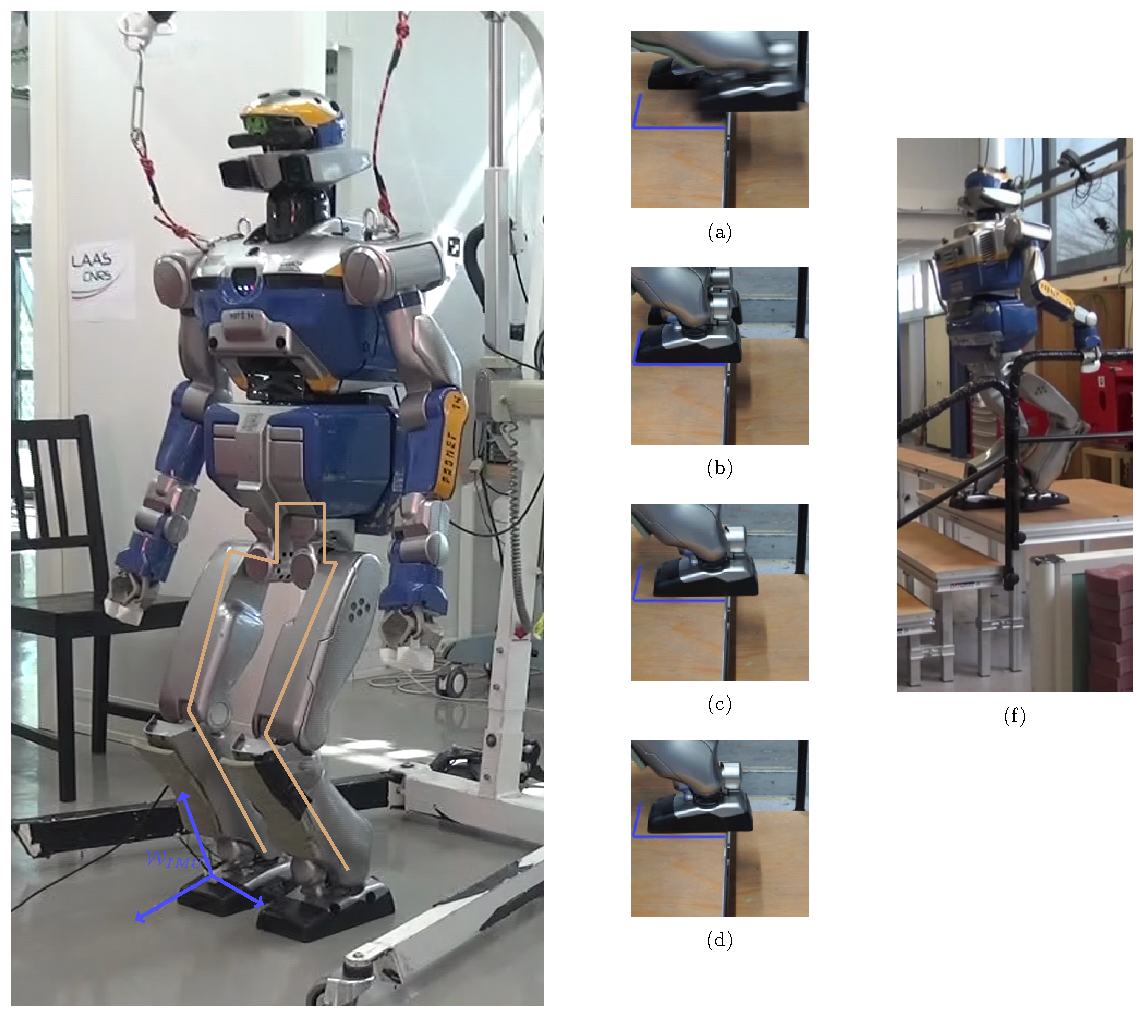
\includegraphics[width=\linewidth]{./figures/cover-figure.pdf}
	\caption{The flying foot trajectory is reconstructed through an IMU set on the foot (in blue), and by fusing the information coming from the kinematic chain
        from the support foot to the flying one (in light brown). In the middle images (a)-(d) shows slippage while performing a multicontacts motion depicted on the
        right (f) (from \cite{Carpentier:ICRA:2016}).
 }
	\label{fig:cover}
\end{figure}

For robots where the design choices introduces flexibilities such as HRP-2 \cite{Nakaoka:iros:2007}, or backlashes,
the system needs a state estimator being able to take into account this uncertainty.
In addition a good pose estimation of the robot in its environment is still needed for effective interactions with the environment,
and especially for behavior involving manipulation or multiple contact locomotion.
This estimation can then be used to compute the commands that will be sent to actuators.
%<<<<<<< HEAD
%Fusion strategies with information coming from different sensors can be used to achieve this goal. 
%Considering the application in a real environment, we can fuse the odometer with a high frequency proprioceptive sensor 
%to get better predictions of robot poses by improving integration points.
%
%Using an IMU (Inertial Measurement Unit) allows us get acceleration and angular velocity measurement that can be used to 
%compute the pose of the robot and get information similar to odometry by integration for the fusion step.
%These sensors are now used in a wide range of applications: aerospace, SLAM, human motion analysis, or robotics.
%
%=======

Localization can be used to perform real-time planning and model predictive control.
To achieve this goal fusion strategies with information coming from different sensors is needed.
Graphical methods have been extensively used to implement such fusion strategies \cite{Thrun:ijrr:2006,Kaess:itro:2008}.
They have been used for large modeling estimation problems by means of sparse networks of constraints. 
In robotics, the problems of visual odometry, and simultaneous localization and mapping, have reached a high degree of maturity, 
in great part thanks of the graphical representation. 
This is so, among other aspects, because of the power of the graphical representation to accurately model complex estimation problems. 
These often involve dynamics, proprioceptive measures, exteroceptive measures, and self-calibration.
The graphical representation also allows for the design of powerful nonlinear estimation solvers, which can be built taking into account the needs for accuracy, 
robustness and CPU-performance.
In order to keep the problem tractable and maintain real-time performance a key point is to avoid the graph to be too large for a given time window.
IMU is challenging in this regards, as its high frequency measurement creates large set of data. 
 
For this reason it was proposed in \cite{LUPTON-09,forster2015imu} to preintegrate the IMU information over an horizon where IMU data are the only
ones to be measured.
A first contribution of this paper is to reformulate the method proposed in \cite{forster2015imu} from rotation matrix to quaternion
and give a detailed and simpler algebraic derivation.
The second contribution is to apply this method to the measurement of a humanoid robot flying foot pose.
The level of accuracy obtained with this approach is allowing us to detect foot slippage. 
Finally we described the implementation of this preintegration scheme in a software implementation of the graphical method.
%>>>>>>> 8a2771fa9c6aae6c3980ef5238504b80af3260c9




